\documentclass[a4paper,12pt]{article}
\usepackage{amsmath}
\usepackage{amsfonts}
\usepackage{amssymb}
\usepackage{graphicx}
\usepackage{tikz}
\usepackage{geometry}
\usepackage{tabularx}
\usepackage{xcolor}
\usepackage{colortbl}
\usepackage{float}
\usetikzlibrary{positioning,shapes.geometric}
\geometry{a4paper, margin=1in}
\usepackage[utf8]{inputenc}
\usepackage[T1]{fontenc}
\usepackage{listings}
\lstset{
  basicstyle=\ttfamily\small,
  breaklines=true,
  breakatwhitespace=true,
  postbreak=\mbox{\textcolor{red}{$\hookrightarrow$}\space},
  language=SQL,
  showspaces=false,
  showstringspaces=false,
  frame=single,
  framesep=2pt,
  framerule=0pt,
  xleftmargin=2pt,
  xrightmargin=2pt,
  columns=flexible,
  tabsize=2,
  commentstyle=\color{gray},
  keywordstyle=\color{blue},
  stringstyle=\color{orange},
  identifierstyle=\color{black},
  morekeywords={INSERT,INTO,VALUES,CREATE,TABLE,ALTER,ADD,SET,FOREIGN,KEY,REFERENCES,UPDATE},
  otherkeywords={--,=>,->,::},
  deletekeywords={ACCESS,KEY}
  }

\title{Database Design for Privat Transport}
\author{University Exam}
\date{\today}
\begin{document}
\maketitle

\section*{Introduction}
This document details the database design process for Privat Transport, a private transport company established in Grimstad in 2023. The design follows a structured methodology comprising conceptual, logical, and physical database design phases. The objective is to create a database application to support the operations of Privat Transport, addressing issues of information sharing and administrative efficiency.

\section*{Conceptual Database Design}
The conceptual database design involves constructing a model of the data requirements independent of physical considerations. The steps include identifying entity types, relationship types, attributes, and keys, and validating the model against user transactions.

\subsection*{Step 1.1: Identify Entity Types}
\begin{table}[H]
\centering
\begin{tabularx}{\textwidth}{|X|}
\hline
\rowcolor{blue!20} \textbf{Entity Types} \\
\hline
Office \\
\hline
Manager \\
\hline
CarOwner \\
\hline
Driver \\
\hline
AdministrativeStaff \\
\hline
Car \\
\hline
PrivateClient \\
\hline
BusinessClient \\
\hline
Contract \\
\hline
Job \\
\hline
\end{tabularx}
\end{table}

\subsection*{Step 1.2: Identify Relationship Types}
\begin{table}[H]
\centering
\begin{tabularx}{\textwidth}{|X|}
\hline
\rowcolor{blue!20} \textbf{Relationship Types} \\
\hline
Manager Manages Office \\
\hline
CarOwner Owns Car \\
\hline
Driver Drives Car \\
\hline
Office Employs AdministrativeStaff \\
\hline
PrivateClient Requests Job \\
\hline
BusinessClient Has Contract \\
\hline
Contract Includes Job \\
\hline
Job AssignedTo Driver \\
\hline
Job Uses Car \\
\hline
\end{tabularx}
\end{table}

\subsection*{Step 1.3: Identify and Associate Attributes}
\begin{table}[H]
\centering
\begin{tabularx}{\textwidth}{|X|X|}
\hline
\rowcolor{blue!20} \textbf{Entity} & \textbf{Attributes} \\
\hline
Office & officeID, city \\
\hline
Manager & managerID, name, phone, officeID \\
\hline
CarOwner & ownerID, name, phone \\
\hline
Driver & driverID, name, sex, DOB, phone, officeID \\
\hline
AdministrativeStaff & staffID, name, phone, officeID \\
\hline
Car & carID, registrationNo, model, ownerID \\
\hline
PrivateClient & clientID, name, phone, address \\
\hline
BusinessClient & clientID, name, phone, address \\
\hline
Contract & contractID, clientID, numberOfJobs, fee \\
\hline
Job & jobID, clientID, contractID, pickUpDateTime, pickUpAddress, dropOffAddress, mileage, charge, status \\
\hline
\end{tabularx}
\end{table}

\subsection*{Step 1.4: Determine Attribute Domains}
\begin{table}[H]
\centering
\begin{tabularx}{\textwidth}{|X|X|}
\hline
\rowcolor{blue!20} \textbf{Attribute} & \textbf{Domain} \\
\hline
officeID & Integer \\
\hline
managerID, ownerID, driverID, staffID, clientID, contractID, jobID & Integer \\
\hline
name, phone, address, model, registrationNo & String \\
\hline
sex & Char (M, F) \\
\hline
DOB, pickUpDateTime & Date \\
\hline
numberOfJobs, mileage & Integer \\
\hline
fee, charge & Decimal \\
\hline
status & String (Completed, Failed) \\
\hline
\end{tabularx}
\end{table}

\subsection*{Step 1.5: Determine Candidate, Primary, and Alternate Key Attributes}
\begin{table}[H]
\centering
\begin{tabularx}{\textwidth}{|X|X|}
\hline
\rowcolor{blue!20} \textbf{Entity} & \textbf{Primary Key} \\
\hline
Office & officeID \\
\hline
Manager & managerID \\
\hline
CarOwner & ownerID \\
\hline
Driver & driverID \\
\hline
AdministrativeStaff & staffID \\
\hline
Car & carID \\
\hline
PrivateClient & clientID \\
\hline
BusinessClient & clientID \\
\hline
Contract & contractID \\
\hline
Job & jobID \\
\hline
\end{tabularx}
\end{table}

\subsection*{Step 1.6: Consider Use of Enhanced Modeling Concepts (Optional)}
\begin{table}[H]
\centering
\begin{tabularx}{\textwidth}{|X|}
\hline
\rowcolor{blue!20} \textbf{Enhanced Modeling Concepts} \\
\hline
Specialization: Client superclass with PrivateClient and BusinessClient subclasses. \\
\hline
\end{tabularx}
\end{table}

\subsection*{Step 1.7: Check Model for Redundancy}
\begin{table}[H]
\centering
\begin{tabularx}{\textwidth}{|X|}
\hline
\rowcolor{blue!20} \textbf{Redundancy Check} \\
\hline
Ensure no redundant entities or relationships exist. \\
\hline
\end{tabularx}
\end{table}

\subsection*{Step 1.8: Validate Conceptual Model Against User Transactions}
\begin{table}[H]
\centering
\begin{tabularx}{\textwidth}{|X|}
\hline
\rowcolor{blue!20} \textbf{Validation} \\
\hline
Validate that the model supports all user transactions such as listing managers, female drivers, total staff, car details, etc. \\
\hline
\end{tabularx}
\end{table}

\subsection*{Step 1.9: Review Conceptual Data Model with User}
\begin{table}[H]
\centering
\begin{tabularx}{\textwidth}{|X|}
\hline
\rowcolor{blue!20} \textbf{Review} \\
\hline
Review the ER diagram and associated documentation with the user. \\
\hline
\end{tabularx}
\end{table}

For this step we would simply review if the ER diagram below encompasses the requirements from the them. 

\begin{figure}[!ht]
\centering
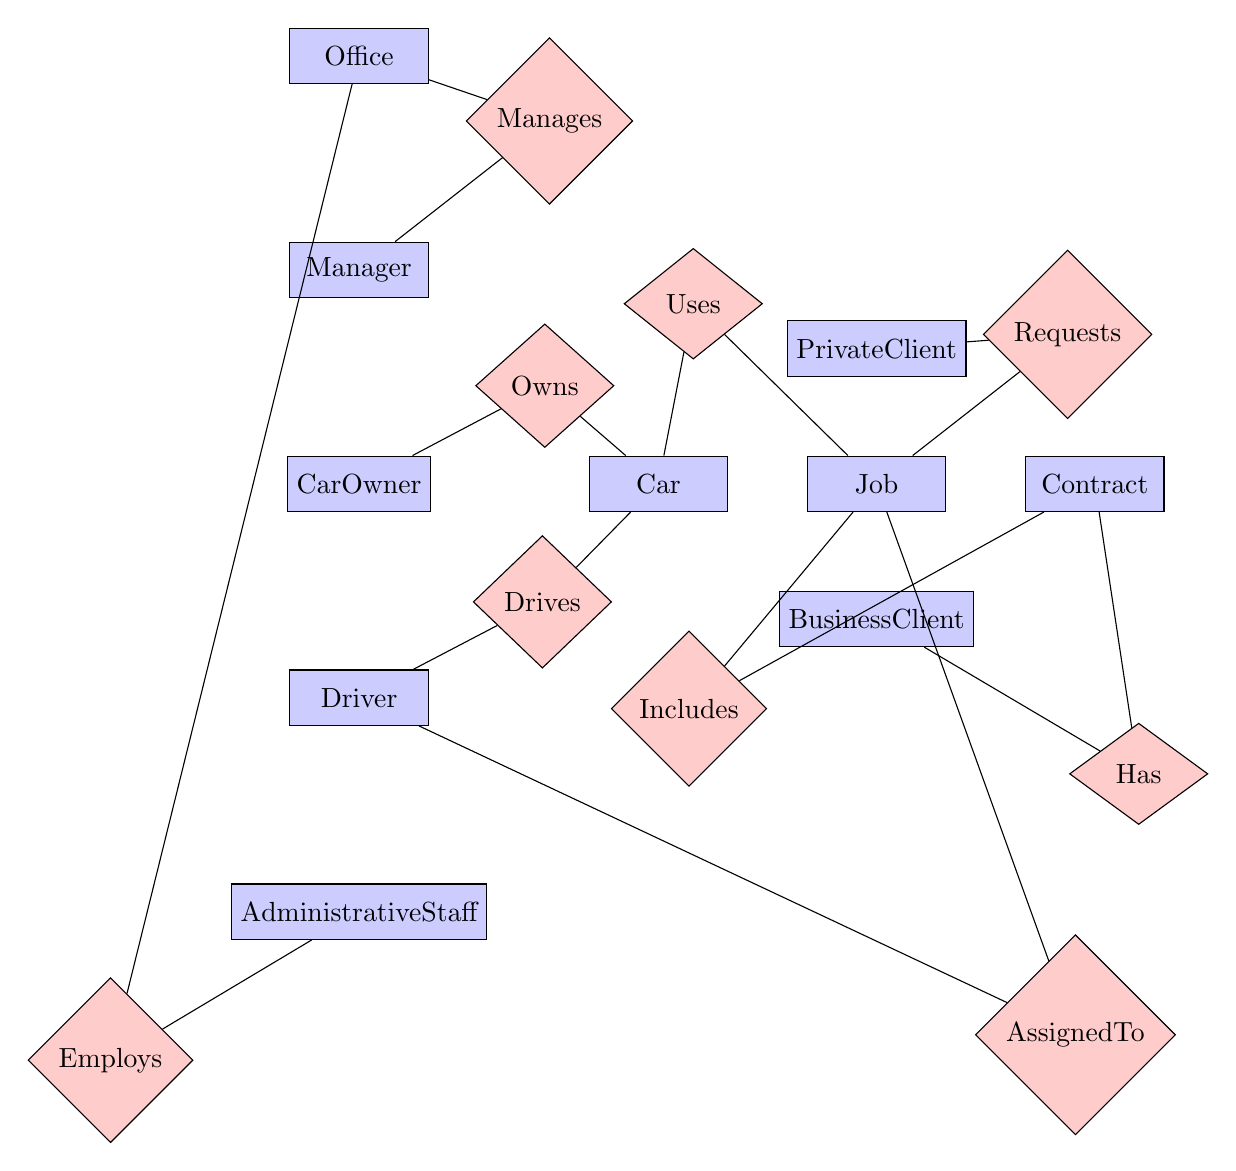
\begin{tikzpicture}[node distance=2cm, every node/.style={fill=white,draw}]
  \tikzset{
    entity/.style={draw, rectangle, minimum height=2em, minimum width=5em, text centered, fill=blue!20},
    relationship/.style={draw, diamond, minimum height=2em, minimum width=5em, text centered, fill=red!20}
  }

  \node[entity] (office) {Office};
  \node[entity, below=of office] (manager) {Manager};
  \node[entity, below=of manager] (owner) {CarOwner};
  \node[entity, below=of owner] (driver) {Driver};
  \node[entity, below=of driver] (staff) {AdministrativeStaff};
  \node[entity, right=2cm of owner] (car) {Car};
  \node[entity, right=1cm of car] (job) {Job};
  \node[entity, above=1cm of job] (pclient) {PrivateClient};
  \node[entity, below=1cm of job] (bclient) {BusinessClient};
  \node[entity, right=1cm of job] (contract) {Contract};

  \node[relationship, above right=1cm and 1cm of manager] (manages) {Manages};
  \node[relationship, below right=-2cm and 1cm of owner] (owns) {Owns};
  \node[relationship, below right=-2cm and 1cm of driver] (drives) {Drives};
  \node[relationship, below left=1cm and 1cm of staff] (employs) {Employs};
  \node[relationship, above right=1cm and 1cm of job] (requests) {Requests};
  \node[relationship, below right=3cm and 2cm of job] (has) {Has};
  \node[relationship, below left=2cm and 1cm of job] (includes) {Includes};
  \node[relationship, below right=6cm and 1cm of job] (assignedto) {AssignedTo};
  \node[relationship, below left=-3cm and 1cm of job] (uses) {Uses};

  \draw (office) -- (manages);
  \draw (manages) -- (manager);
  \draw (owner) -- (owns);
  \draw (owns) -- (car);
  \draw (driver) -- (drives);
  \draw (drives) -- (car);
  \draw (office) -- (employs);
  \draw (employs) -- (staff);
  \draw (pclient) -- (requests);
  \draw (requests) -- (job);
  \draw (bclient) -- (has);
  \draw (has) -- (contract);
  \draw (contract) -- (includes);
  \draw (includes) -- (job);
  \draw (job) -- (assignedto);
  \draw (assignedto) -- (driver);
  \draw (job) -- (uses);
  \draw (uses) -- (car);
\end{tikzpicture}
\caption{ER Diagram for Privat Transport}
\end{figure}

\newpage

\section*{Logical Database Design}
The logical database design translates the conceptual data model into a relational model. The steps include deriving relations, validating them using normalization, and ensuring they support user transactions.

\subsection*{Step 2.1: Derive Relations for Logical Data Model}
\begin{table}[H]
\centering
\begin{tabularx}{\textwidth}{|X|}
\hline
\rowcolor{green!20} \textbf{Relations for Logical Data Model} \\
\hline
Office(officeID, city) \\
\hline
Manager(managerID, name, phone, officeID) \\
\hline
CarOwner(ownerID, name, phone) \\
\hline
Driver(driverID, name, sex, DOB, phone, officeID) \\
\hline
AdministrativeStaff(staffID, name, phone, officeID) \\
\hline
Car(carID, registrationNo, model, ownerID) \\
\hline
PrivateClient(clientID, name, phone, address) \\
\hline
BusinessClient(clientID, name, phone, address) \\
\hline
Contract(contractID, clientID, numberOfJobs, fee) \\
\hline
Job(jobID, clientID, contractID, pickUpDateTime, pickUpAddress, dropOffAddress, mileage, charge, status) \\
\hline
\end{tabularx}
\end{table}

\subsection*{Step 2.2: Validate Relations Using Normalization}
\begin{table}[H]
\centering
\begin{tabularx}{\textwidth}{|X|}
\hline
\rowcolor{green!20} \textbf{Normalization Validation} \\
\hline
Ensure all relations are in at least Third Normal Form (3NF) to eliminate redundancy and ensure data integrity. \\
\hline
\end{tabularx}
\end{table}

\subsection*{Step 2.3: Validate Relations Against User Transactions}
\begin{table}[H]
\centering
\begin{tabularx}{\textwidth}{|X|}
\hline
\rowcolor{green!20} \textbf{User Transaction Validation} \\
\hline
Check that each relation supports the necessary user transactions. \\
\hline
\end{tabularx}
\end{table}

\subsection*{Step 2.4: Define Integrity Constraints}
\begin{table}[H]
\centering
\begin{tabularx}{\textwidth}{|X|}
\hline
\rowcolor{green!20} \textbf{Integrity Constraints} \\
\hline
Ensure all primary keys, foreign keys, and other constraints are correctly defined. \\
\hline
\end{tabularx}
\end{table}

\subsection*{Step 2.5: Review Logical Data Model with User}
\begin{table}[H]
\centering
\begin{tabularx}{\textwidth}{|X|}
\hline
\rowcolor{green!20} \textbf{Review} \\
\hline
Review the logical data model with the user for accuracy and completeness. \\
\hline
\end{tabularx}
\end{table}

\begin{figure}[!ht]
\centering
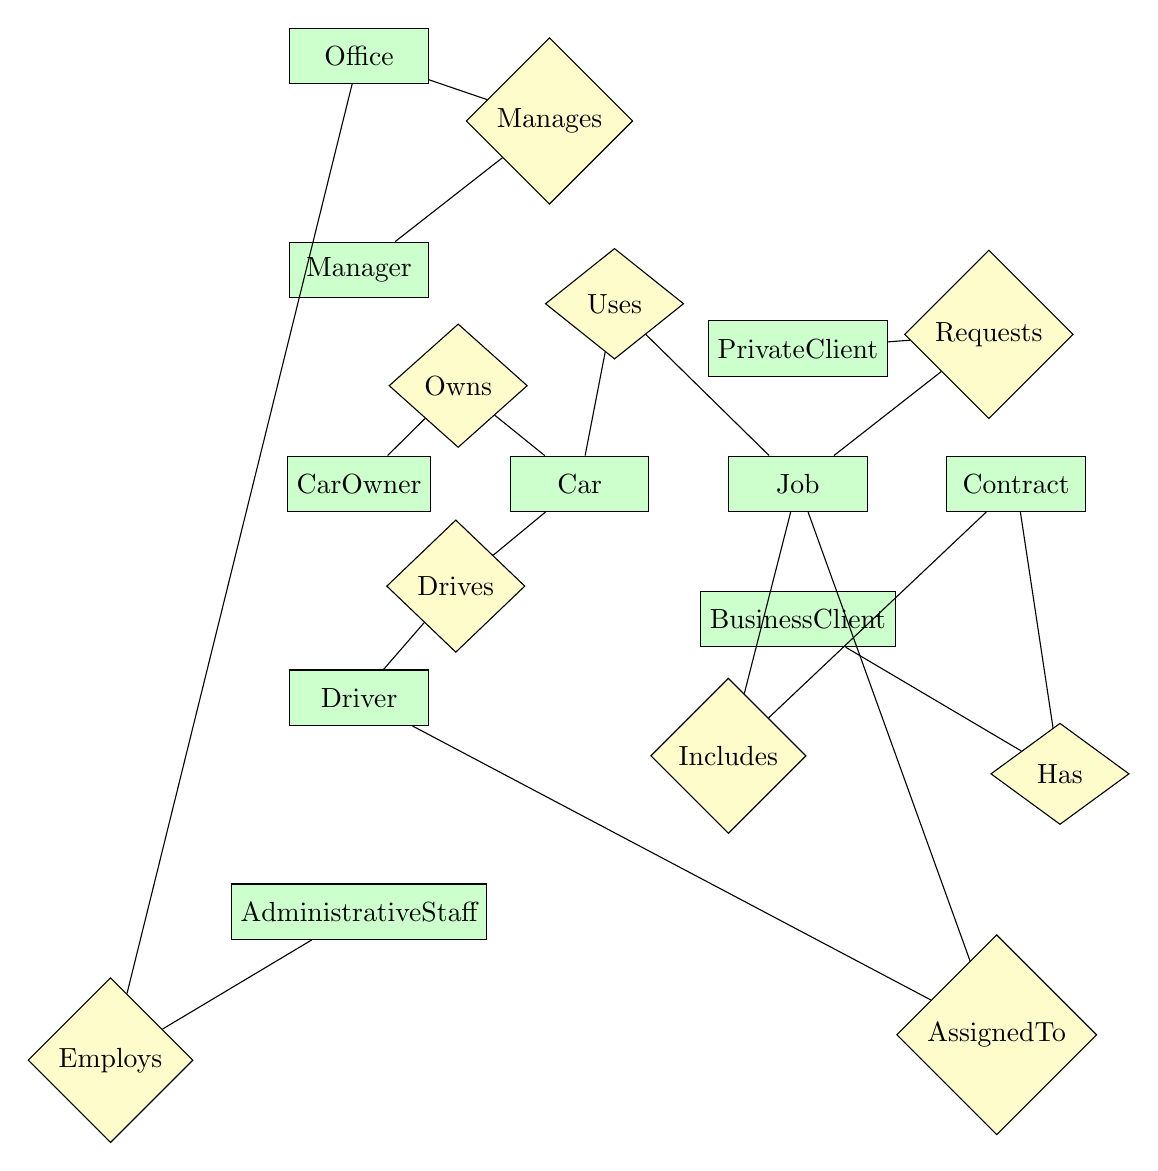
\begin{tikzpicture}[node distance=2cm, every node/.style={fill=white,draw}]
  \tikzset{
    entity/.style={draw, rectangle, minimum height=2em, minimum width=5em, text centered, fill=green!20},
    relationship/.style={draw, diamond, minimum height=2em, minimum width=5em, text centered, fill=yellow!20}
  }

  \node[entity] (office) {Office};
  \node[entity, below=of office] (manager) {Manager};
  \node[entity, below=of manager] (owner) {CarOwner};
  \node[entity, below=of owner] (driver) {Driver};
  \node[entity, below=of driver] (staff) {AdministrativeStaff};
  \node[entity, right=1cm of owner] (car) {Car};
  \node[entity, right=1cm of car] (job) {Job};
  \node[entity, above=1cm of job] (pclient) {PrivateClient};
  \node[entity, below=1cm of job] (bclient) {BusinessClient};
  \node[entity, right=1cm of job] (contract) {Contract};

  \node[relationship, above right=1cm and 1cm of manager] (manages) {Manages};
  \node[relationship, below right=-2cm and -0.1cm of owner] (owns) {Owns};
  \node[relationship, below right=-2.2cm and -0.1cm of driver] (drives) {Drives};
  \node[relationship, below left=1cm and 1cm of staff] (employs) {Employs};
  \node[relationship, above right=1cm and 1cm of job] (requests) {Requests};
  \node[relationship, below right=3cm and 2cm of job] (has) {Has};
  \node[relationship, below left=2.6cm and -0.5cm of job] (includes) {Includes};
  \node[relationship, below right=6cm and 1cm of job] (assignedto) {AssignedTo};
  \node[relationship, below left=-3cm and 1cm of job] (uses) {Uses};

  \draw (office) -- (manages);
  \draw (manages) -- (manager);
  \draw (owner) -- (owns);
  \draw (owns) -- (car);
  \draw (driver) -- (drives);
  \draw (drives) -- (car);
  \draw (office) -- (employs);
  \draw (employs) -- (staff);
  \draw (pclient) -- (requests);
  \draw (requests) -- (job);
  \draw (bclient) -- (has);
  \draw (has) -- (contract);
  \draw (contract) -- (includes);
  \draw (includes) -- (job);
  \draw (job) -- (assignedto);
  \draw (assignedto) -- (driver);
  \draw (job) -- (uses);
  \draw (uses) -- (car);
\end{tikzpicture}
\caption{ER Diagram for Logical Data Model}
\end{figure}

\newpage

\section*{Physical Database Design}
The physical database is simply a physical implementation on MySQL. This below is the SQL schema and constraints.

\subsection*{Step 3.1: Translate Logical Data Model for MySQL}
Here there is 3 scripts \\
scripts for each table based on the logical data model.
scripts for populating the model.\\
scripts for running transactions.\\

lastly there is the simple terminal test app.


\subsection*{SQL Implementation}

\subsubsection*{SQL Scripts for Creating the Database and Tables}
\begin{lstlisting}[language=SQL]
CREATE TABLE Office (
    officeID INT PRIMARY KEY,
    city VARCHAR(100)
);

CREATE TABLE Manager (
    managerID INT PRIMARY KEY,
    name VARCHAR(100),
    phone VARCHAR(15),
    officeID INT,
    FOREIGN KEY (officeID) REFERENCES Office(officeID)
);

CREATE TABLE CarOwner (
    ownerID INT PRIMARY KEY,
    name VARCHAR(100),
    phone VARCHAR(15)
);

CREATE TABLE Driver (
    driverID INT PRIMARY KEY,
    name VARCHAR(100),
    sex CHAR(1),
    DOB DATE,
    phone VARCHAR(15),
    officeID INT,
    FOREIGN KEY (officeID) REFERENCES Office(officeID)
);

CREATE TABLE AdministrativeStaff (
    staffID INT PRIMARY KEY,
    name VARCHAR(100),
    phone VARCHAR(15),
    officeID INT,
    FOREIGN KEY (officeID) REFERENCES Office(officeID)
);

CREATE TABLE Car (
    carID INT PRIMARY KEY,
    registrationNo VARCHAR(10),
    model VARCHAR(50),
    ownerID INT,
    FOREIGN KEY (ownerID) REFERENCES CarOwner(ownerID)
);

CREATE TABLE PrivateClient (
    clientID INT PRIMARY KEY,
    name VARCHAR(100),
    phone VARCHAR(15),
    address VARCHAR(255)
);

CREATE TABLE BusinessClient (
    clientID INT PRIMARY KEY,
    name VARCHAR(100),
    phone VARCHAR(15),
    address VARCHAR(255)
);

CREATE TABLE Contract (
    contractID INT PRIMARY KEY,
    clientID INT,
    numberOfJobs INT,
    fee DECIMAL(10,2),
    FOREIGN KEY (clientID) REFERENCES BusinessClient(clientID)
);

CREATE TABLE Job (
    jobID INT PRIMARY KEY,
    clientID INT,
    contractID INT,
    pickUpDateTime DATETIME,
    pickUpAddress VARCHAR(255),
    dropOffAddress VARCHAR(255),
    mileage INT,
    charge DECIMAL(10,2),
    status VARCHAR(20),
    FOREIGN KEY (clientID) REFERENCES PrivateClient(clientID),
    FOREIGN KEY (contractID) REFERENCES Contract(contractID)
);
\end{lstlisting}

\subsubsection*{SQL Scripts for Populating the Database}
\begin{lstlisting}[language=SQL]
    -- Populate Office
    INSERT INTO Office (officeID, city) VALUES (1, 'Grimstad'), (2, 'Oslo'), (3, 'Bergen');
    
    -- Populate Manager
    INSERT INTO Manager (managerID, name, phone, officeID) VALUES 
    (1, 'John Doe', '12345678', 1),
    (2, 'Jane Smith', '23456789', 2),
    (3, 'Emily Davis', '34567890', 3);
    
    -- Populate CarOwner
    INSERT INTO CarOwner (ownerID, name, phone) VALUES 
    (1, 'Alice Johnson', '45678901'),
    (2, 'Robert Brown', '56789012');
    
    -- Populate Driver
    INSERT INTO Driver (driverID, name, sex, DOB, phone, officeID) VALUES 
    (1, 'Michael Clark', 'M', '1980-01-01', '67890123', 1),
    (2, 'Sarah Lewis', 'F', '1985-02-02', '78901234', 2);
    
    -- Populate AdministrativeStaff
    INSERT INTO AdministrativeStaff (staffID, name, phone, officeID) VALUES 
    (1, 'Olivia Martinez', '89012345', 1),
    (2, 'Liam Wilson', '90123456', 2);
    
    -- Populate Car
    INSERT INTO Car (carID, registrationNo, model, ownerID) VALUES 
    (1, 'AB12345', 'Toyota', 1),
    (2, 'BC23456', 'Honda', 2);
    
    -- Populate PrivateClient
    INSERT INTO PrivateClient (clientID, name, phone, address) VALUES 
    (1, 'Noah Moore', '12345678', '123 Street, Grimstad');
    
    -- Populate BusinessClient
    INSERT INTO BusinessClient (clientID, name, phone, address) VALUES 
    (1, 'TechCorp', '23456789', '456 Avenue, Oslo');
    
    -- Populate Contract
    INSERT INTO Contract (contractID, clientID, numberOfJobs, fee) VALUES 
    (1, 1, 10, 5000.00);
    
    -- Populate Job
    INSERT INTO Job (jobID, clientID, contractID, pickUpDateTime, pickUpAddress, dropOffAddress, mileage, charge, status) VALUES 
    (1, 1, NULL, '2023-05-01 10:00:00', '789 Boulevard, Bergen', '123 Street, Grimstad', 10, 100.00, 'Completed'),
    (2, 1, 1, '2023-05-02 11:00:00', '456 Avenue, Oslo', '789 Boulevard, Bergen', 20, NULL, 'Completed');
    
\end{lstlisting}

\subsubsection*{SQL Scripts for Running Transactions}
\begin{lstlisting}[language=SQL]
    -- Transaction to find names and phone numbers of the Managers at each office
    SELECT name, phone FROM Manager;
    
    -- Transaction to find names of all female drivers based in the Grimstad office
    SELECT name FROM Driver WHERE sex = 'F' AND officeID = 1;
    
    -- Transaction to find total number of staff at each office
    SELECT officeID, COUNT(*) AS total_staff FROM 
    (
        SELECT officeID FROM Manager 
        UNION ALL 
        SELECT officeID FROM Driver 
        UNION ALL 
        SELECT officeID FROM AdministrativeStaff
    ) AS staff
    GROUP BY officeID;
    
    -- Transaction to find details of all cars at the Grimstad office
    SELECT carID, registrationNo, model FROM Car WHERE ownerID IN (SELECT ownerID FROM CarOwner WHERE officeID = 1);    
\end{lstlisting}

\subsubsection*{simple console app}
\begin{verbatim}
    using System;
    using MySql.Data.MySqlClient;
    
    class Program
    {
        static void Main()
        {
            string connectionString = "Server=localhost;Database=PrivatTransport;User ID=root;Password=password;";
            using (MySqlConnection conn = new MySqlConnection(connectionString))
            {
                conn.Open();
    
                // Example of inserting a new driver
                string insertDriverQuery = "INSERT INTO Driver (driverID, name, sex, DOB, phone, officeID) VALUES (3, 'Laura Thompson', 'F', '1990-03-03', '34567890', 1)";
                using (MySqlCommand cmd = new MySqlCommand(insertDriverQuery, conn))
                {
                    cmd.ExecuteNonQuery();
                }
    
                // Example of selecting all drivers
                string selectDriversQuery = "SELECT * FROM Driver";
                using (MySqlCommand cmd = new MySqlCommand(selectDriversQuery, conn))
                {
                    using (MySqlDataReader reader = cmd.ExecuteReader())
                    {
                        while (reader.Read())
                        {
                            Console.WriteLine($"{reader["driverID"]}, {reader["name"]}, {reader["sex"]}, {reader["DOB"]}, {reader["phone"]}, {reader["officeID"]}");
                        }
                    }
                }
            }
        }
    }    
\end{verbatim}

\section*{Conclusion}
This report shows the complete database design process for Privat Transport, including conceptual, logical, and physical design phases. The models and SQL scripts provided ensure a robust database implementation suitable for the company's needs.

\newpage
\section*{REFERENCES}
The used references are class documents(pdf, powerpoints etc.) mostly on chapter 16.
\end{document}
